\section{이론적 배경}
%\section{Theoretical Background}

\subsection{조파 수조와 조파기}
조파 수조는 조파기가 달린 모형 실험용 수조로 해안 혹은 연안에서의 여러 현상을 축소하여 재현 및 실험하기 위한 장치이다. 정밀한 실험을 위해서 기업체나 연구실에서는 큰 스케일로 제작하기도 한다. 주로 선박의 안정성이나 연안에 설치한 구조물의 내구성 등을 시험할 때 맞는 환경을 조성해준다. 초기에는 실험적으로 만들어졌으나 유체 관련 연구가 진행되면서 이론적인 분석이 추가되었다. 
%본교에서 제작한 조파 수조는 파의 진행방향이 한 방향이며 2차원 조파 수조라고 부른다. 

소규모로 운영이 용이하며 비교적 정확한 파를 생성하고 변화를 관찰하기 위해서는 파의 진행방향이 한 방향인 2차원 조파 수조가 적합하다. 2차원 조파 수조를 이용하여 파 특성에 관한 기본 연구나 파와 물체 간의 상호작용에 대한 실험 연구를 충분히 수행할 수 있다. 

\begin{figure}[htbp]
\begin{center}
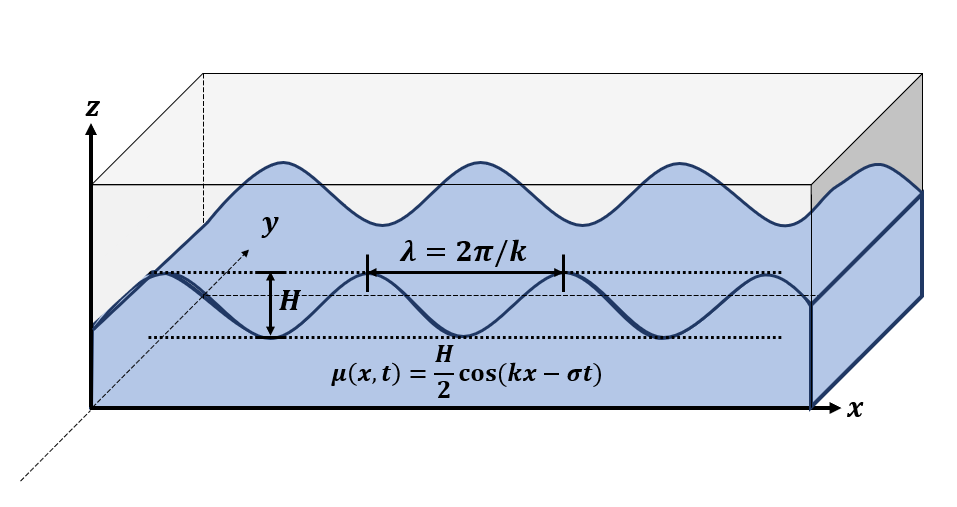
\includegraphics[width=10cm, trim={0 1.8cm 0 1.5cm}, clip]{Water_Tank(Illustrated).png}
\end{center}
\caption{조파 수조 모식도}
\label{Fig01}
\end{figure}
%해파를 만들때 현상을 재현하기 위한 환경을 조성하며 
조파기는 조파 수조에서 파를 생성하는 장치이다. 조파기는 판의 운동 방식에 따라 플랩형, 피스톤형, 플런저형 등이 있다. 피스톤형 조파기는 연안 환경에서의 실험에 자주 사용되는 천해파를 생성하기 용이하다. 피스톤형 조파기에서 파를 생성하는 조파판의 모든 요소는 일관적으로 수평 운동을 한다. 또, 판의 수평 운동 범위를 스트로크라고 하며 $S_0$로 쓰도록 한다 (단, 이는 판의 각 부분이 모두 함께 운동하는 경우에 해당한다).

% 세 종류의 조파기를 보여주는 그림이 필요함.

\subsection{조파 이론(wave maker theory)}

조파 이론은 여러 종류의 조파기가 발생하는 파도의 특성과 개형을 알아보는 것을 목표로 한다\cite{dean1991water} \cite{zhang2007deterministic} \cite{ojk2018}.
2차원 조파 수조에서 피스톤형 조파기가 발생시키는 파도는 여러 방정식을 통해 구할 수 있다. 제일 보편적인 방식은 속도 퍼텐셜 $\phi(x, y, z, t)$를 정의하고 이에 대한 라플라스 방정식과 여러 경계조건을 적용하는 것이다. 방정식을 풀면 속도 퍼텐셜은 다음과 같이 정해진다.

\begin{equation} \label{eq:1}
{
\phi(x, z, t) = A\cosh{[k(h+z)]}\sin(kx-\sigma t) +
\cos(\sigma t){\sum_{n=1}^{\infty}} C_n e^{-k_3 x} \cos{[k_3 (z+h)]} 
}
\end{equation}

%$$\phi(x, z, t) = A\cosh{[k(h+z)]}\sin(kx-\sigma t) + $$
%$$\cos(\sigma t){\sum_{n=1}^{\infty}} C_n e^{-k_3 x} \cos{[k_3 (z+h)]}  $$

파동은 $x$방향으로 진행하며 $h$는 수심이고 $k$는 파수, $\sigma$는 각진동수이다. 그외의 문자는 상수이며 식(\ref{eq:1})로부터 발생파의 변위 식을 다음과 같이 쓸 수 있다.

\begin{equation} \label{eq:2}
{
\mu(x, t) = {{1 \over g}{{\partial \phi} \over {\partial t}}|_{z=0} } = \frac{A \sigma}{g} \cosh(kh) \cos(kx-\sigma t) +
\sin(\sigma t) {\sum_{n=1}^{\infty}} \frac{\sigma C_n}{g} e^{-k_3 x} \cos(k_3 h)
}
\end{equation}

%$$\mu(x, t) = \frac{A \sigma}{g} \cosh(kh) \cos(kx-\sigma t) + $$
%$$\sin(\sigma t) {\sum_{n=1}^{\infty}} \frac{\sigma C_n}{g} e^{-k_3 x} cos(k_3 h) $$

식 (\ref{eq:1}), (\ref{eq:2}) 모두 첫 항은 진행파, 두 번째 항은 정상파를 의미한다. 정상파의 $k_3$은 진팽파의 분산관계식을 정상파 파수로 변환한 식에서 구할 수 있으며 $\sigma ^2 = -g k_3 \tan{k_3 h}$의 해이다. 하지만 제일 큰 해에 대해서 감쇠되는 비율 $\exp{(-k_{3}x)}$가 $x=2h$일 때 $0.04$, $x=3h$일 때 0.009 수준으로 급감하며 본 연구에서는 수조 길이가 6$m$, 수심이 약 15$cm$ 수준이므로 정상파는 무시할 수 있다. 또, 미분방정식의 각각의 고유함수에 대해 일차 근사를 적용하여 파고 $H$를 다음과 같이 표현할 수 있다.

\begin{equation} \label{eq:4}
H = \frac{4 S_0 \sin h{kh}}{\sin h{2kh}+2kh} \left(\sin h{k[z_d - h]} - \sin h{k[z_u - h]}\right)
\end{equation}

%$$H = \frac{4 S_0 \sin h{kh}}{\sin h{2kh}+2kh} (\sin h{k[z_d - h]} - \sin h{k[z_u - h]}) $$

$z_d$는 조파판 하단의 깊이, $z_u$는 조파판 상단의 깊이이며 본 연구의 경우 조파판이 수심 전체에 걸쳐 존재하므로 $z_d = h$, $z_u = 0$이고 파고와 파동 함수는 다음과 같다.

\begin{equation} \label{eq:5}
{
    \frac{H}{S_0}=\frac{4 \sinh^2 k h}{\sinh 2kh + 2kh}
     = \frac{4 \sinh^2 z}{\sinh 2z+2 z}, ~z=kh
}
\end{equation}

\begin{equation} \label{eq:6}
{
    \mu(x, t)=\frac{H}{2} \cos (k x-\sigma t)
}
\end{equation}

%$$\frac{H}{S_0}=\frac{4 \sinh ^2 k h}{\sinh k h+2 k h}, \mu(x, t)=\frac{H}{2} \cos (k x-\sigma t)$$

$S_0,~h$는 구조적인 값이며 조절이 가능하다. 또, 파수 $k$와 각진동수 $\sigma$는 분산 관계식을 만족하므로 결론적으로는 $\sigma$와 $S_0$, $h$를 정하면 된다. 조파판 또한 sin형으로 움직이도록 경계조건으로 반영되었으며 이 경우 판의 진동 변위는 다음과 같다.

\begin{equation} \label{eq:7}
{
    x = {{S_0}\over2} \sin{\sigma t}
}
\end{equation}

하지만 이는 심해파의 경우이다. 여러 경계조건과 근사를 하기 위한 조건이며 심해파는 간단하게 $h/\lambda > 1/2$인 파를 의미하기도 한다. 이와 반대로 천해파는 $h/\lambda < 1/20$인 파를 의미하며 상대적으로 얕은 바다에서 생기며 파가 진행하면서 부서진다. 그렇기 때문에 이론적으로 파의 개형을 해석적으로 유도하기는 거의 불가능하며 대부분의 선행연구는 섭동이론을 적용하거나 2차까지 근사를 하는 등 비선형으로 방정식을 수치해석한다\cite{society1993laboratory}. 

\subsection{소파 장치(wave absorber)}
파는 수조 내부에서 전달되며 진행파와 주변 장애물에 부딫혀 반사된 반사파로 나뉜다. 중첩의 원리에 의하여 수면파는 진행파와 반사에 의한 정상파의 선형 결합으로 표현되며 정상파가 주요 오차의 원인이 된다. 소파기는 반사파가 생기지 않도록 해주는 장치로 능동형 소파 장치(active wave absorber)\와 수동형 소파 장치(passive wave absorber)로 나뉜다\cite{ouellet1986survey}.

%\subsubsection{능동형 소파기}

능동형 소파 장치는 또 다른 조파기가 있어서 벽에 입사하는 파를 완전히 상쇄시킬 수 있는 파를 만들어 반사하지 않도록 하는 것이다. 벽에 입사하는 파의 개형을 실시간으로 측정하여 이에 맞는 파를 발생시킬 수 있어야 하며 상당히 고가의 장비이고 사용가능한 환경, 구조가 제한되어 있다. 이는 벽 부근에 다른 조파기를 설치하는 방식이며 파를 발생하는 조파기가 자체적으로 운동을 제어하여 반사파를 상쇄시키도록 움직일 수도 있다. 이는 '흡수 조파' 방식으로 조파판에서 파의 개형을 측정하여 반사파를 상쇄하는 파를 추가적으로 생성하는 것이다.

%\subsubsection{수동형 소파기(passive wave absorber)}

수동형 소파 장치는 추가적인 구조물을 설치하여 반사파의 에너지를 최소화하는 것을 목적으로 한다. 능동형 소파 장치와 달리 아무리 최적화를 해도 반사파가 존재하며 horsehair, crushed rock 등 여러 구조가 있다. 특히, 파를 효과적으로 소멸시키기 위해 다공성 판을 이용하며 공극률에 따른 반사계수 비교 등 다공성 구조 관련 연구가 많으며 이미 그 효율성이 입증되었다\cite{lim2014optimum, o2017methods}. 또, 경사로를 이용하기도 하는데 이는 주로 3D 조파 수조에서 파를 관찰하려는 영역이 아닌 다른 부분에서 최대한 상쇄시키기 위함이다. 경사로는 위로 볼록한 포물면을 띄는 경우가 제일 반사계수가 낮음이 밝혀졌다. 본 연구에서는 수동형 소파기를 사용할 것이다.

\subsection{파고계(wave gauge)}

파고계는 파도의 높이(파고)를 재기 위한 측정 장치이다. 측정 방식에 따라 용량식, 저항식, 수압식, 초음파식 등여러 종류로 나뉘며 사용하는 장소의 규모, 정밀도에 따라 달라진다. 본 연구에서는 저항형 파고계를 사용하려고 하였으나 제대로 측정이 되지 않았다. 핵심원리는 물에 잠긴 와이어의 깊이에 따라서 전기전도도가 달라지고 저항이 바뀌는 점을 이용하여 전류값과 수심을 대응시키는 것이다. 하지만 실제로 실험을 해본 결과 수심이 $20\mathrm{~cm}$가 바뀔동안 전류가 $0.1\mathrm{~A}$가 바뀌었으며 이 값이 최소눈금이다. 전류 증폭을 시도해보았으나 회로가 버틸 수 있는 범위 내에서는 측정을 할 수 없으며 결국 부표를 띄우고 영상을 찍어 파도의 파고 데이터를 얻어내는 방식을 채택하였다.

\subsection{Froude 상사 법칙}
모형실험을 하는 경우 축척이 달라지면 물리적 특성이 바뀐다. 이때 무차원 수가 보존되어야 한다는 원리가 Froude 상사 법칙이며 보존되는 무차원 수를 Froude 수라고 한다.\cite{briggs2013basics, chakrabarti1994offshore} 이외에도 Reynolds 수, Prandtl 수 등이 보존되기도 하나 본 실험의 경우 액체의 점성이나 확산보다는 파의 진행에 초점을 맞추기 때문에 Froude 수가 보존되는 경우를 생각한다. Froude 수는 다음과 같이 정의된다.
\begin{equation}
    Fr = \frac{V}{\sqrt{gL}}
\end{equation}

$V$는 움직이는 개체(파도; 물, 배, 비행기 등)의 속도이며 $g$는 중력가속도, $L$은 계의 특성길이이다. 수조와 바다에 대한 Froude 수가 같아야 하며 두 계 모두 움직이는 개체는 파도이기 때문에 분산 관계식을 이용하여 새롭게 쓸 수 있다.

\begin{equation}
    Fr = \sqrt{\frac{\tanh{kh}}{kL}}
\end{equation}

특성 길이는 단면이 직사각형이 수조의 경우 $L = {2ab}/{(a+b)}$임이 알려져 있으며 $a$는 수조의 폭, $b$는 수조 내 물의 수심이다. 바다의 경우 이를 근사적으로 $2h$로 생각할 수 있다 ($h$는 바다의 수심이다). $a=30\mathrm{~cm}, b=15\mathrm{~cm}$를 대입하여 관계식을 구해보면 다음과 같다.

\begin{quote}
    \[f(z_i) = \frac{\tanh{z_i}}{z_i},~  z_i = k_i h_i\]

    \begin{multicols}{2}

    계 1: 수조
    \[{Fr_1}^{2} = \frac{a+b}{2ab} \frac{\tanh{k_1 b}}{k_1} = \frac{3}{4} f(z_{1})\]

    \columnbreak
    
    계 2: 깊은 바다
    \[{Fr_2}^{2} = \frac{1}{2h_2} \frac{\tanh{k_2 h_2}}{k_2} = \frac{1}{2} f(z_{2})\]
    \end{multicols}

\end{quote}

\begin{equation}
    \therefore \frac{3}{2}f(z_1 ) = f(z_2 )
\end{equation}

$z_i = 2\pi h_i/\lambda_i$이므로 심해파, 천해파의 경계값(각각 $h/\lambda = 1/2, 1/20$)을 대입해보면 모형 실험의 경우 천해파는 $\omega \sim \pi$이고 심해파는 $\omega \sim 4\pi$ 정도는 되어야 한다는 결론을 내릴 수 있다. 단, 이는 수조의 수심이 $15\mathrm{~cm}$인 경우이며 더 깊어져도 약 $20\mathrm{~cm}$정도가 최대이고 얕아진다고 한들 $\omega$는 각각 $\pi$, $4\pi$ 정도는 되어야 한다.




